% !TeX program = lualatex
% !TeX encoding = utf8
% !BIB program = biber
% !TeX spellcheck = uk_UA
% chktex-file 2, 3, 12, 24

\documentclass{mathreport}
% ------------------------------------------------------------------------------------------------------------
% Add Additional Packages
% ------------------------------------------------------------------------------------------------------------

\renewcommand{\theequation}{\arabic{subsection}.\arabic{equation}}
\renewcommand{\thesubsection}{\arabic{subsection}}

\usepackage{bbm} % for using indicator \mathbbm{1}

% reset equation numbering after each subsection
\counterwithin*{equation}{subsection}

% set page background color (dark read mode)
% \pagecolor[rgb]{0.118,0.118,0.118}
% \color[rgb]{0.8,0.8,0.8}

\begin{document}

\ReportName{Домашнє завдання №2}

\import{Title/}{title}

\tableofcontents

\newpage
\section{Щільність розподілу енергії}
% \addcontentsline{toc}{section}{Розподіл функції від однієї неперервної випадкової величини}

\setcounter{subsection}{1}
\setcounter{equation}{0}

Нехай задано таку функціональну залежність значень енергії~$E$ та температури~$T$:
\begin{equation}\label{eq: energy intro}
    E(T) = A + B\tanh{\left( \frac{T-T_0}{C} \right)},
\end{equation}
де значення~$A$, $B$, $C$ та $T_0$ в рамках фізичної моделі є константами. Тепер нехай покладемо величину~$C$ як неперервно розподілену нормальну випадкову величну з математичним сподіванням~$\mu_c$ та дисперсією~$\sigma_c$:
\begin{equation}\label{eq: C coefficient distribution}
    C \sim \mathrm{N}(\mu_c,\sigma_c^2),
\end{equation}
а отже, щільність розподілу введеної випадкової величини буде такою:
\begin{equation}\label{eq: C explicit coefficient distribution}
    f_C(x) = \frac{1}{\sqrt{2\pi \sigma_c^2}}\, e^{-\frac{(x-\mu_c)^2}{2\sigma_c^2}}
\end{equation}

Відтак, енергія~$E$ матиме функціональну залежність~\eqref{eq: energy intro} від випадкової величини~$C$, де значення~$T$, $T_0$, $A$ та $B$ є фіксованими:
\begin{equation}\label{eq: g(C) intro}
    g(C) = A + B\tanh{\left( \frac{T-T_0}{C} \right)}
\end{equation}

Таким чином, з'ясуємо безпосередній вигляд щільности~$f_E(y)$ випадкової величини~$E$ як результату перетворень, заданих формулою~\eqref{eq: g(C) intro}:
\begin{equation}\label{eq: energy distribution intro}
    E \sim f_E(y)
\end{equation}

За формулою заміни змінних:
\begin{equation}\label{eq: сhange of variables formula}
    f_E(y) = f_C\left( g^{-1}(y) \right) \cdot \left| \frac{d}{dy}g^{-1}(y) \right|,
\end{equation}
де обернена залежність~$g^{-1}(y)$ задаватиметься виразом
\begin{equation}\label{eq: inverse g(y)}
    g^{-1}(y) = \frac{2(T-T_0)}{\ln{(B-A+y)} - \ln{(B+A-y)}},
\end{equation}
а Якобіан перетворення, відповідно, матиме вид
\begin{equation}\label{eq: Jacobian}
    \frac{d}{dy}g^{-1}(y) = -2(T-T_0) \cdot \left( \ln{\frac{B-A+y}{B+A-y}} \right)^{-2} \cdot \frac{2B}{(B-A+y)(B+A-y)}
\end{equation}

Тоді щільність розподілу~$f_E(y)$ записуватиметься так:
\begin{multline*}\label{eq: energy distribution}
    f_E(y) = \frac{1}{\sqrt{2\pi \sigma_c^2}} \cdot \exp{\left[ -\frac{1}{2\sigma_c^2} \left( \frac{2(T-T_0)}{\ln{(B-A+y)} - \ln{(B+A-y)}} - \mu_c \right)^2 \right]} \times \\ 
    \times \left| \left( \ln{\frac{B-A+y}{B+A-y}} \right)^{-2} \cdot \frac{4B(T-T_0)}{(B-A+y)(B+A-y)} \right| \stepcounter{equation}\tag{\theequation}
\end{multline*}

\subsection*{Експериментальний тест №1}
\addcontentsline{toc}{subsection}{Експериментальний тест №1}

Для перевірки коректності наведених викладок порівняємо гістограму значень функції~$g(C)$ симуляції~$N=10\,000$ значень випадкової величини~$C$ та аналітичну криву щільності випадкової величини~$E$~\eqref{eq: energy distribution}. Першим тестом зафіксуємо значення параметрів, ігноручи фізичну інтерпретацію (Табл. \ref{table: Test 1: naive overview}). На Рис.~\ref{pic: Test 1: naive overview} зображено відповідні <<результати життєздатності>> аналітичного розподілу.

\vspace{0.4cm}
\begin{figure}[H]\centering
    \center{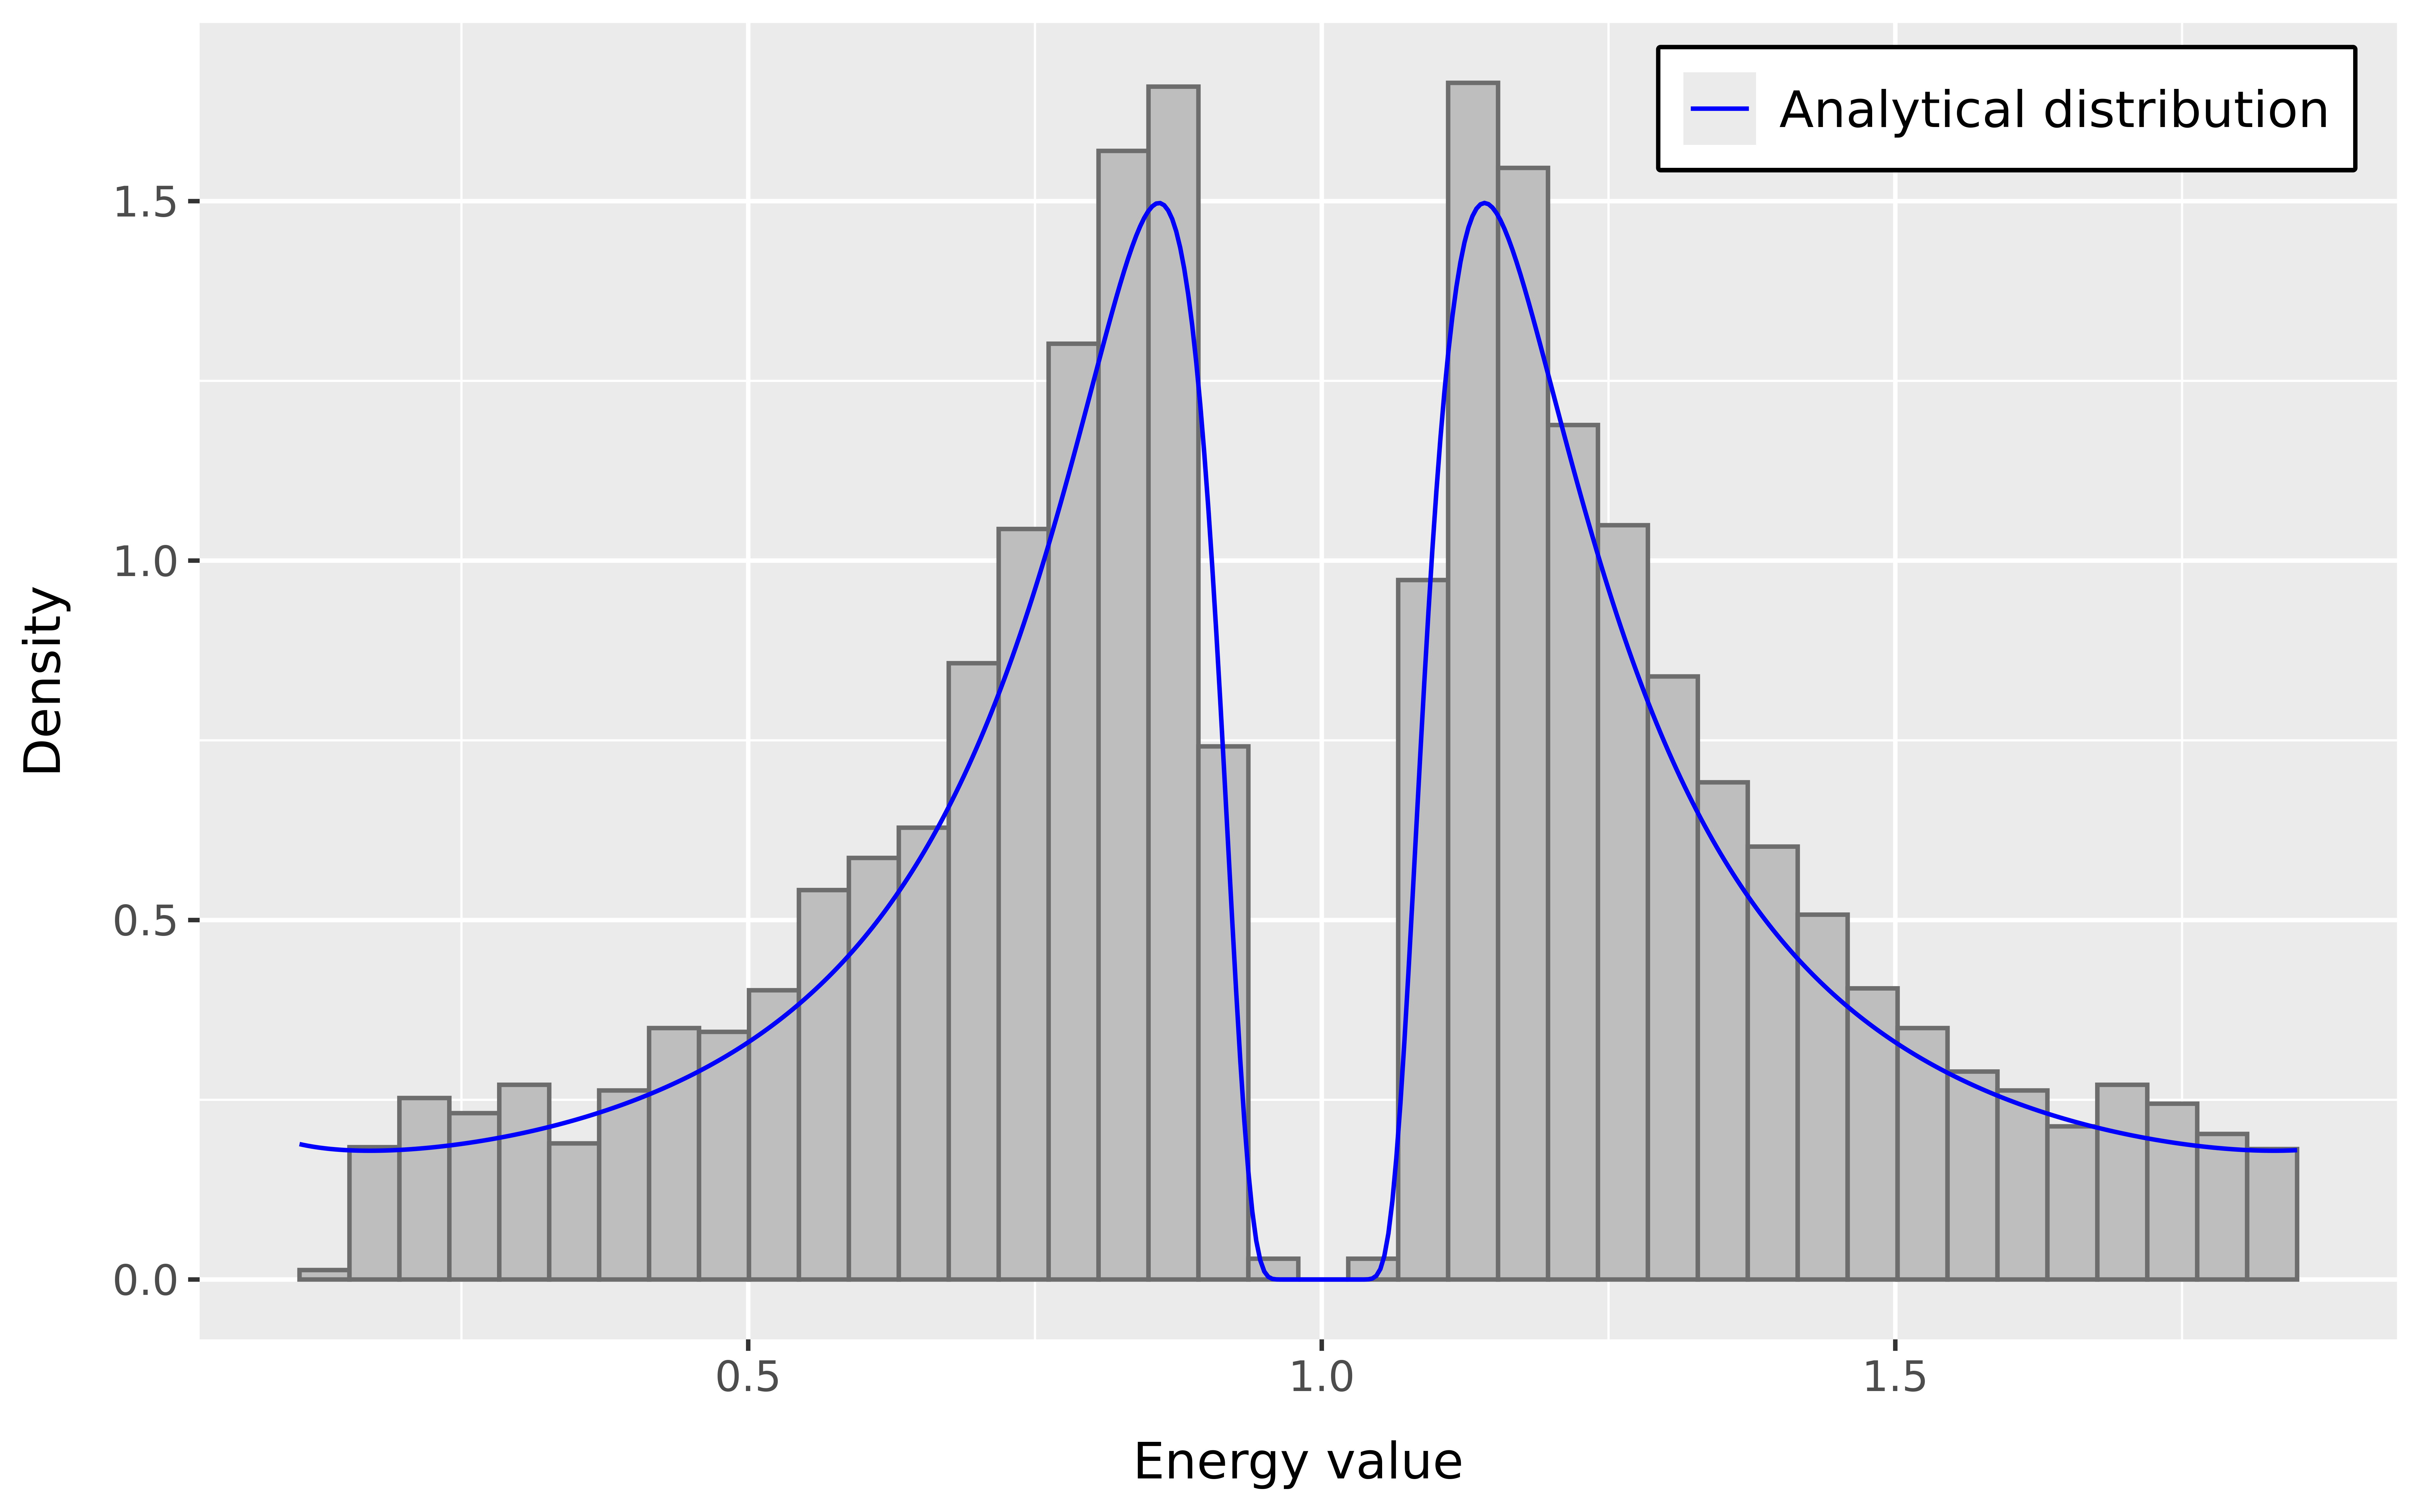
\includegraphics[width=\linewidth]{Images/Test №1: naive overview}}
    \caption{Порівняльний графік симуляції та аналітичного розподілу (Табл.~\ref{table: Test 1: naive overview})}
    \label{pic: Test 1: naive overview}
\end{figure}

\vspace{0.4cm}
\begin{table}[H]\centering
    \begin{tblr}{
            hlines={1pt,solid}, 
            vlines={1pt,solid},
            % hline{4-6}={1-5}{0pt},
            colspec={X[c]X[c]X[c]X[c]X[c]X[c]},
            % cell{1}{1}={r=2,c=1}{c},
            % cell{1}{2}={r=1,c=2}{c},
            % cell{1}{4}={r=1,c=2}{c},
            row{1-2}={mode=math},
        }

        \mu_c & \sigma_c & A  & B  & T  & T_0  \\
        0     & 5        & 1  & 1  & 2  & 1    \\

    \end{tblr}
    \caption{Значення параметрів (без фізичного контексту)}
    \label{table: Test 1: naive overview}
\end{table}

\subsection*{Експериментальний тест №2}
\addcontentsline{toc}{subsection}{Експериментальний тест №2}

Наступним тестом спробуємо зафіксувати значення параметрів з огляду на фізичний зміст. До прикладу~\cite[розділ 3, Табл. 4]{Switzner2023}, використовуючи значення $A=46.4 \pm 6.7$, $B=51.5 \pm 8.0$, $C=18.9 \pm 5.9$ та $T_0=-64.5 \pm 3.5$ було отримано довірчий інтервал~$T_{85}=-46\pm 20$ для відповідного значення енергії~$E=85$. Спробуємо інтерпретувати цей приклад в рамках нашої задачі (Табл.~\ref{table: Test 2: naive phisical contex}). Отримані результати зображені на Рис.~\ref{pic: Test 2: naive phisical contex}.

\vspace{0.4cm}
\begin{figure}[H]\centering
    \center{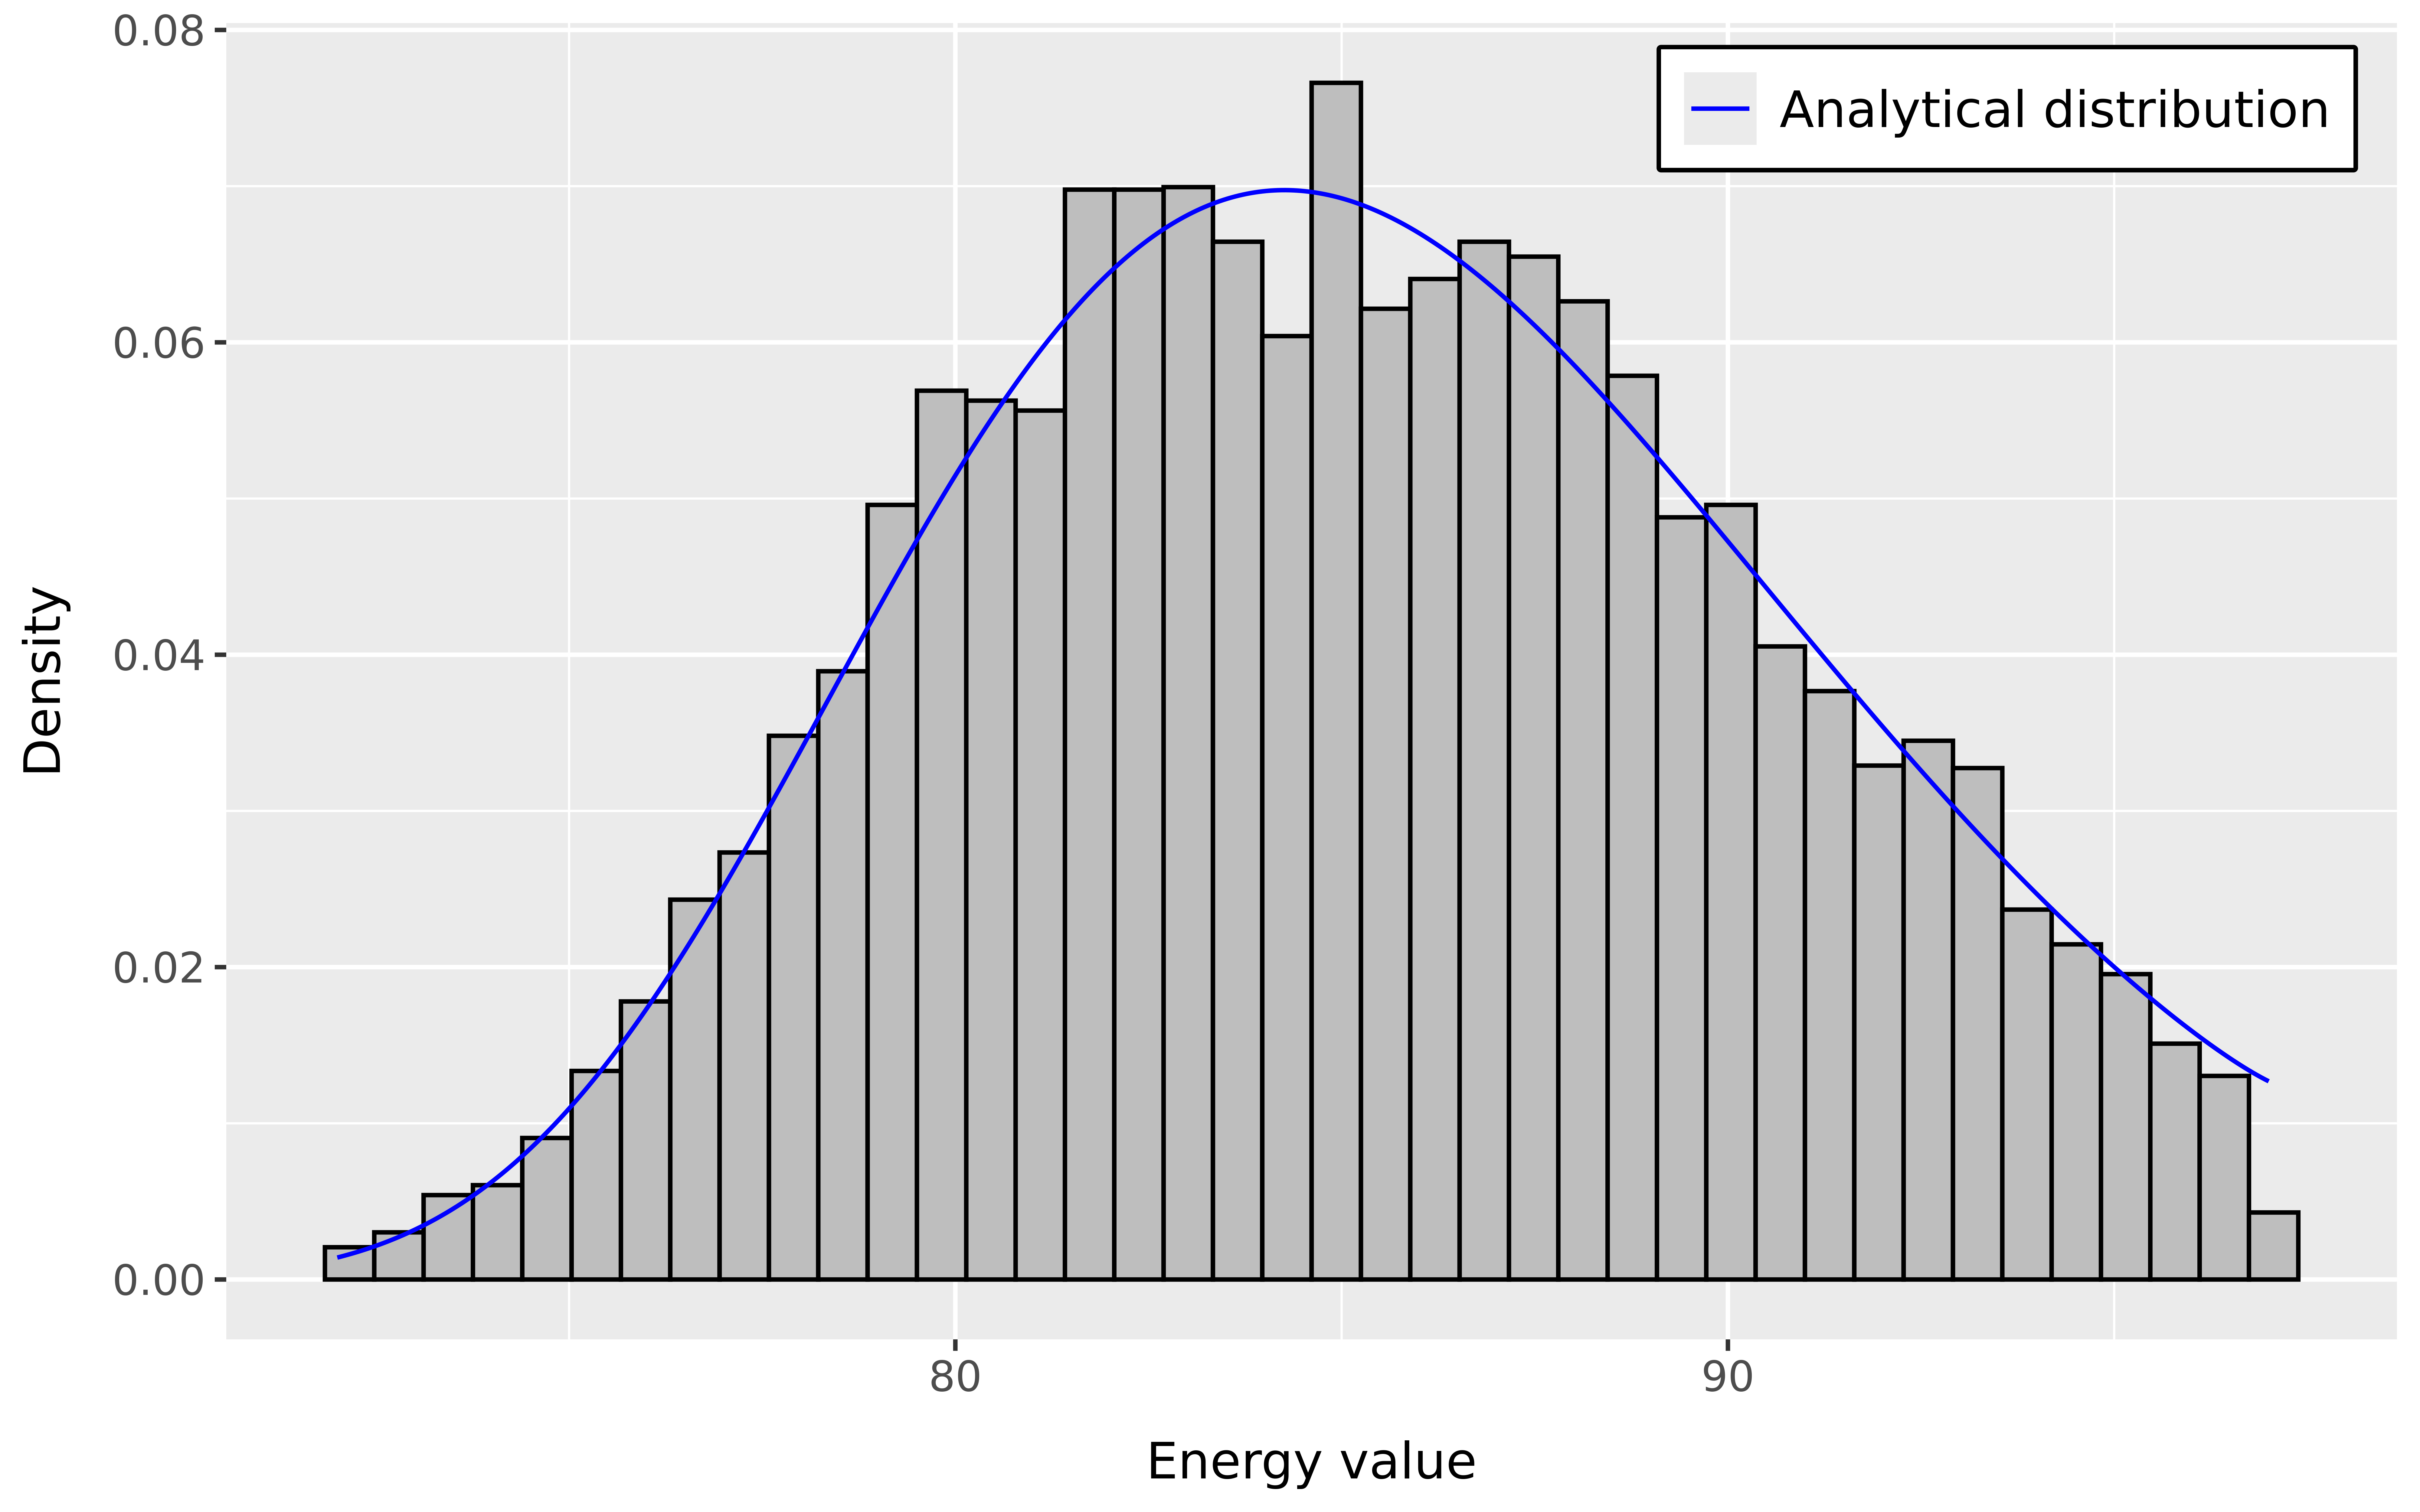
\includegraphics[width=\linewidth]{Images/Test №2: naive phisical contex.png}}
    \caption{Порівняльний графік симуляції та аналітичного розподілу (Табл.~\ref{table: Test 2: naive phisical contex})}
    \label{pic: Test 2: naive phisical contex}
\end{figure}

\vspace{0.4cm}
\begin{table}[H]\centering
    \begin{tblr}{
            hlines={1pt,solid}, 
            vlines={1pt,solid},
            % hline{4-6}={1-5}{0pt},
            colspec={X[c]X[c]X[c]X[c]X[c]X[c]},
            % cell{1}{1}={r=2,c=1}{c},
            % cell{1}{2}={r=1,c=2}{c},
            % cell{1}{4}={r=1,c=2}{c},
            row{1-2}={mode=math},
        }

        \mu_c & \sigma_c & A    & B    & T     & T_0   \\
        18.9  & 5.0      & 46.4 & 51.5 & -46.0 & -64.5 \\

    \end{tblr}
    \caption{Значення параметрів (з огляду на приклад~\cite[розділ 3, Табл. 4]{Switzner2023})}
    \label{table: Test 2: naive phisical contex}
\end{table}

\subsection*{Експериментальний тест №3}
\addcontentsline{toc}{subsection}{Експериментальний тест №3}

Ще один тест проведемо для дещо інших значень параметрів (Табл.~\ref{table: Test 3: phisical contex for each T-value}), при цьому коефіцієнти~$A$ та~$B$ визначимо через~$U$ та~$L$ таким чином:
\begin{equation}\label{eq: L-U denotation}
    A = \frac{U+L}{2},\ B = \frac{U-L}{2}
\end{equation}

Крім того, зобразимо розподіл енергії для~$12$ різних точок температури~$T$, рівновіддалено розподілених на проміжку від~$-90$ до~$0$ (Рис.~\ref{pic: Test 3: phisical contex for each T-value}). 

\vspace{0.4cm}
\begin{table}[H]\centering
    \begin{tblr}{
            hlines={1pt,solid}, 
            vlines={1pt,solid},
            % hline{4-6}={1-5}{0pt},
            colspec={X[c]X[c]X[c]X[c]X[c]},
            % cell{1}{1}={r=2,c=1}{c},
            % cell{1}{2}={r=1,c=2}{c},
            % cell{1}{4}={r=1,c=2}{c},
            row{1-2}={mode=math},
        }

        \mu_c & \sigma_c & L   & U    & T_0   \\
        15  & 5      & 2 & 210 & -50 \\

    \end{tblr}
    \caption{Значення параметрів (моделювання Монте-Карло)}
    \label{table: Test 3: phisical contex for each T-value}
\end{table}

\begin{figure}[H]\centering
    \center{\includegraphics[width=\linewidth]{Images/Test №3: phisical contex for each T-value.png}}
    \caption{Порівняльний графік симуляції та аналітичного розподілу (Табл.~\ref{table: Test 3: phisical contex for each T-value})}
    \label{pic: Test 3: phisical contex for each T-value}
\end{figure}

\newpage
\section{Метод найменших квадратів}
% \addcontentsline{toc}{section}{Розподіл функції від однієї неперервної випадкової величини}

\setcounter{subsection}{2}
\setcounter{equation}{0}

\subsection*{Модель з глобальною адитивною похибкою}
\addcontentsline{toc}{subsection}{Модель з глобальною адитивною похибкою}

Нехай задана така нелінійна регресійна модель:
\begin{equation}\label{eq: NLS true error energy intro}
    E_i = A + B\tanh{\left( \frac{T_i-T_0}{C} \right)} + \varepsilon_i,\ i=\overline{1,n},
\end{equation}
де значення~$A$, $B$ та $T_0$ є фіксованими (Табл.~\ref{table: NLS parameters}), величина~$C$ є невідомим параметром моделі, а випадкова похибка~$\varepsilon_i$ має нормальний розподіл:
\begin{equation}\label{eq: NLS error distribution}
    \varepsilon_i \sim \mathrm{N}(0,\sigma_c^2),\ i=\overline{1,n}
\end{equation}

Першим кроком згенеруємо вибірку даних~$\left( T_i, E_i \right)_{i=\overline{1,n}}$, на основі якої наступним кроком оцінимо параметр~$C$ за методом найменших квадратів (МНК). Для етапу генерування даних покладемо параметр~$C=\mu_c$.

\vspace{0.4cm}
\begin{table}[H]\centering
    \begin{tblr}{
            hlines={1pt,solid}, 
            vlines={1pt,solid},
            % hline{4-6}={1-5}{0pt},
            colspec={X[c]X[c]X[c]X[c]X[c]},
            % cell{1}{1}={r=2,c=1}{c},
            % cell{1}{2}={r=1,c=2}{c},
            % cell{1}{4}={r=1,c=2}{c},
            row{1-2}={mode=math},
        }

        A   & B   & T_0 & \mu_c & \sigma_c \\
        106 & 104 & -50 & 15    & 5        \\

    \end{tblr}
    \caption{Значення параметрів регресійної моделі}
    \label{table: NLS parameters}
\end{table}

У рамках задачі фокус зосереджений навколо~$12$ точкових значень температури~$T$, рівновіддалено розподілених на проміжку $[-90,0]$. Таким чином, організуємо генерування даних так: збиратимемо по $k$ спостережень на кожну з $12$ досліджуваних точок, тобто в результаті матимемо вибірку даних розміром~$n=12k$. Такий підхід дозволить спостерігати за результатами МНК при збільшенні розміру вибірки.

Отже, на основі наявної згенерованої вибірки розміром~$n=12k$ маємо змогу обчислити оцінку параметра~$C$ методом МНК. Для більш наочної картини проведемо серію з $N=10\,000$ повторних запусків МНК для щоразу інших згенерованих даних згідно моделі~\eqref{eq: NLS true error energy intro}. 

Виконаємо аналогічні обчислення при розмірі вибірки в межах кожного запуску МНК як~$n=12$, $n=120$ та~$n=1200$, тобто при генеруванні~$k=1$, $k=10$ та~$k=100$ спостережень на кожну фокус-точку, відповідно. Графіки гістограм оцінок параметра~$C$ продемонстровано на Рис.~\ref{pic: NLS true error results}. З Табл.~\ref{table: NLS true error results} бачимо, що зі збільшенням розміру вибірки~$n$ МНК демонструє збіжні властивості. 

\vspace{0.4cm}
\begin{figure}[H]
    \begin{minipage}[H]{0.32\linewidth}
        \center{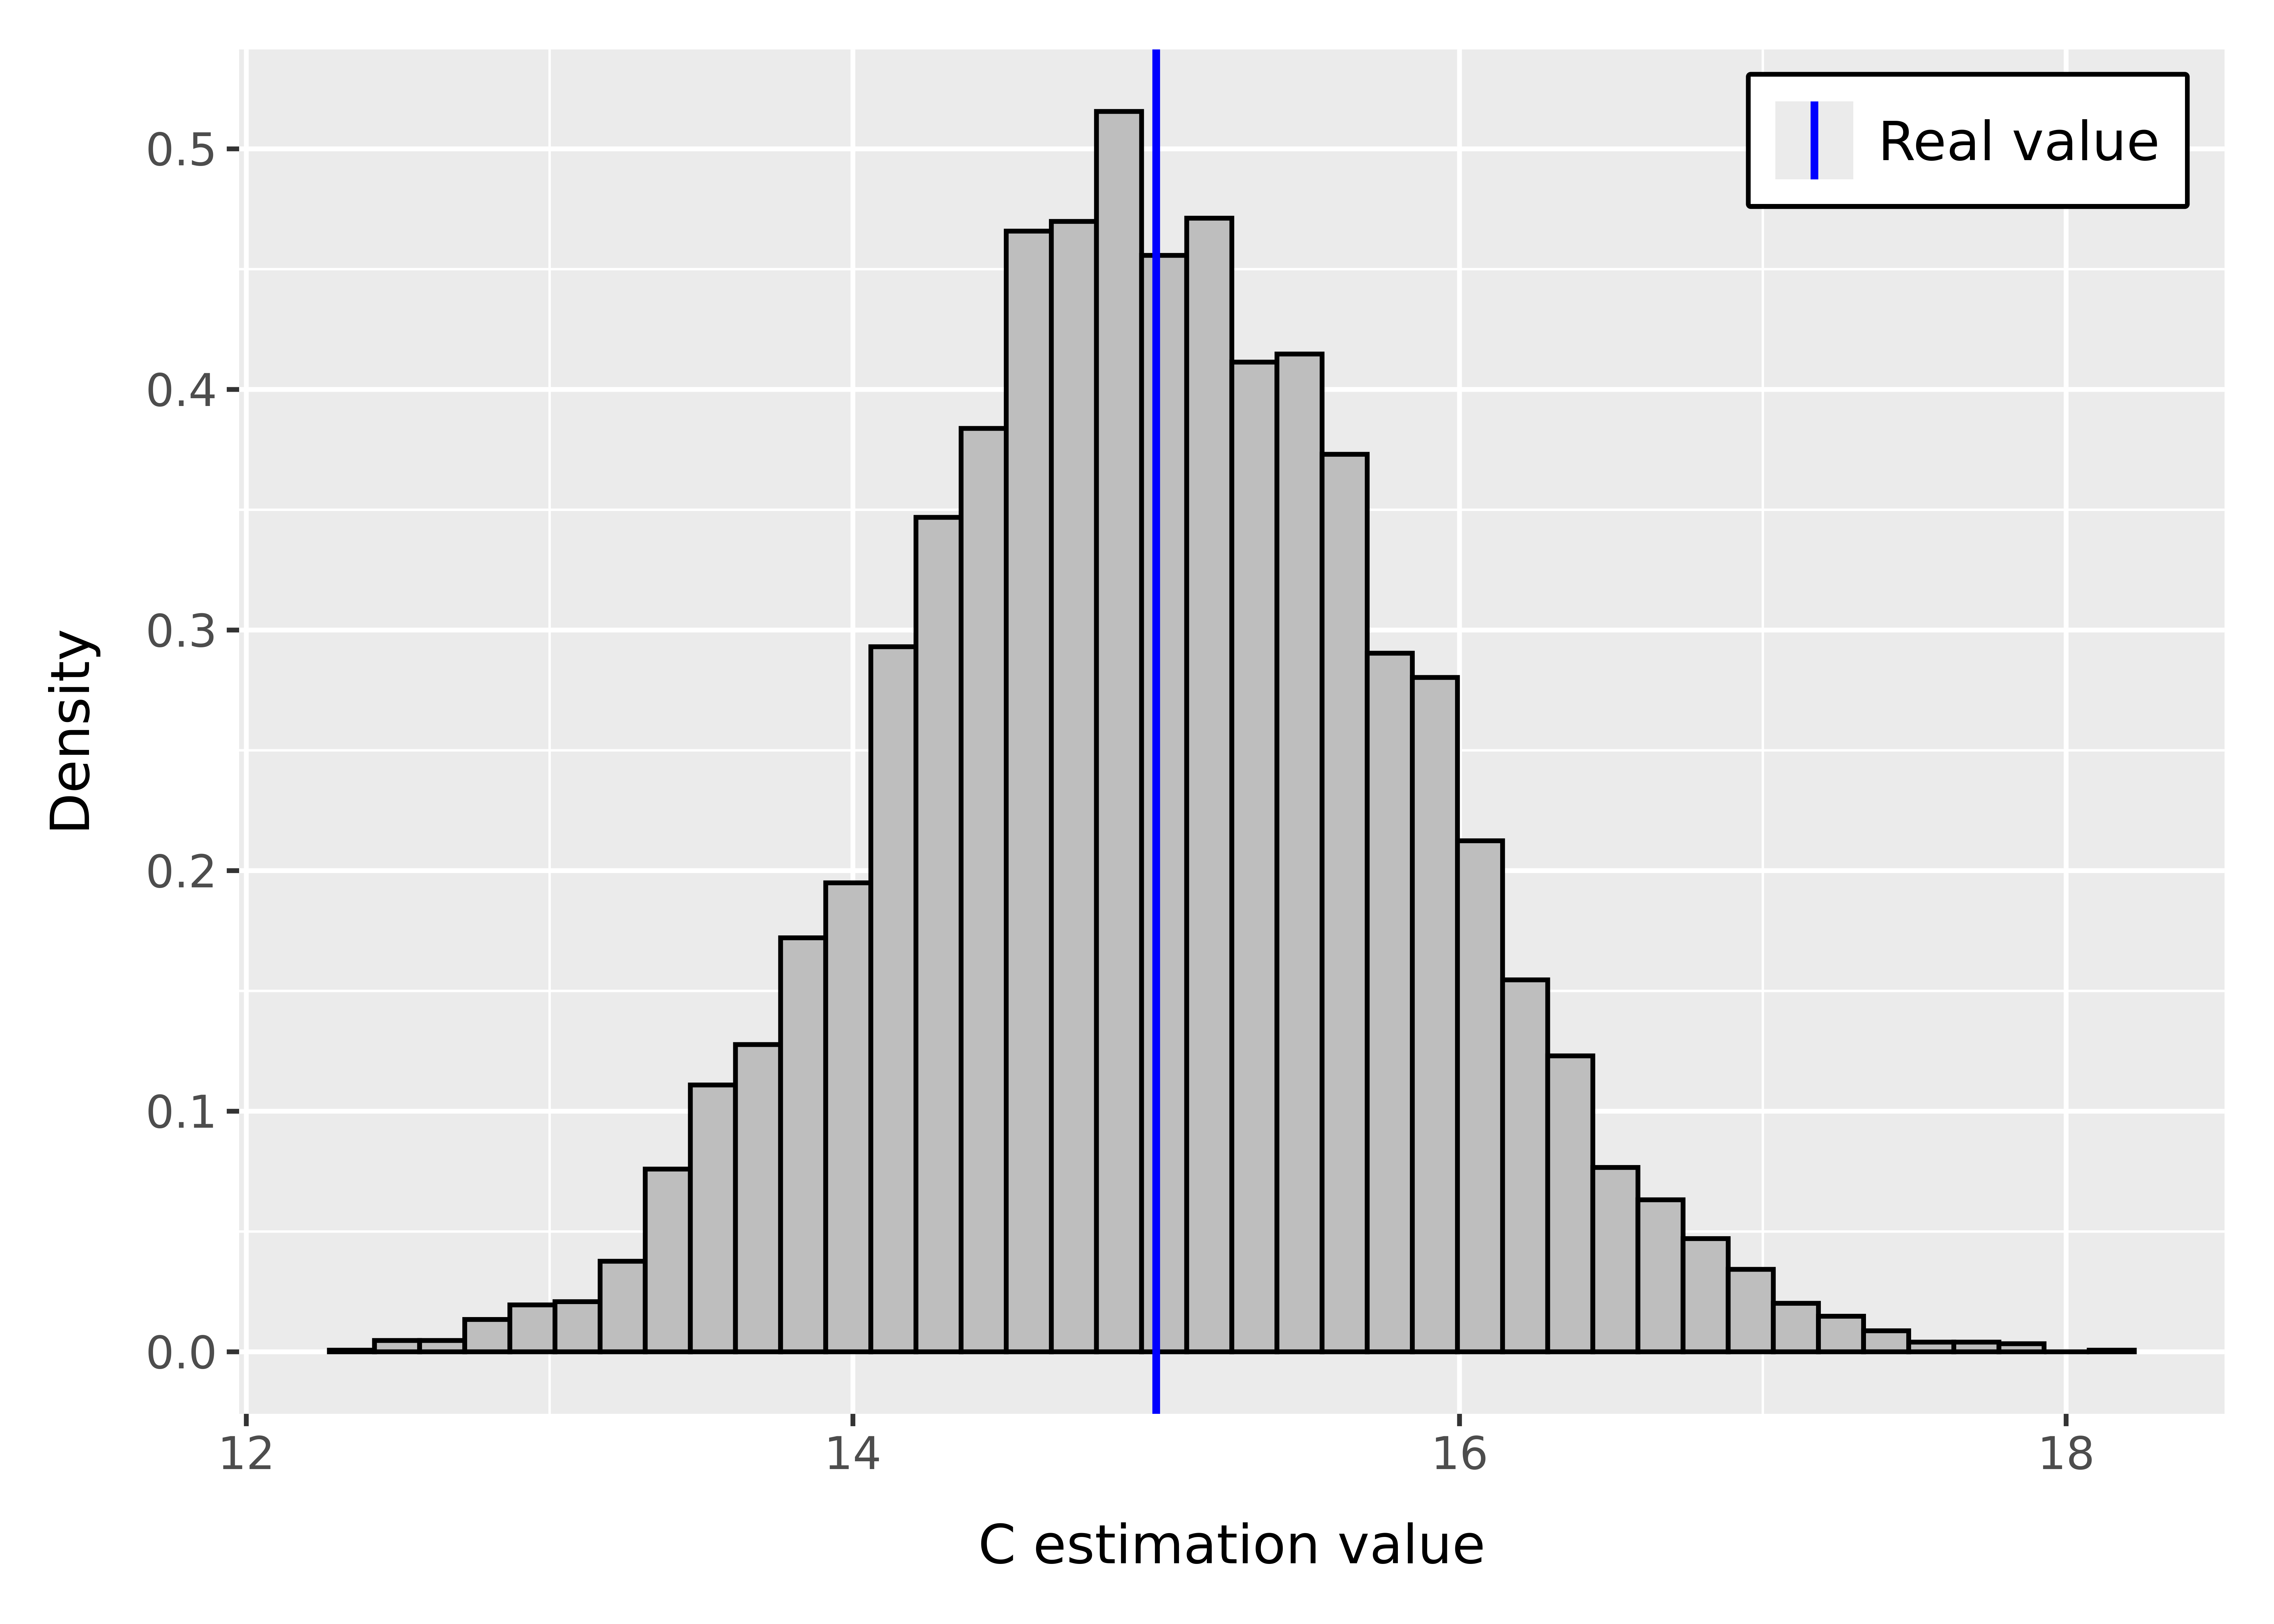
\includegraphics[width=1\linewidth]{Images/TRUE ERROR: NLS regression, n = 12.png}} а) Вибірка $n=12$
    \end{minipage}
    \hfill
    \begin{minipage}[H]{0.32\linewidth}
        \center{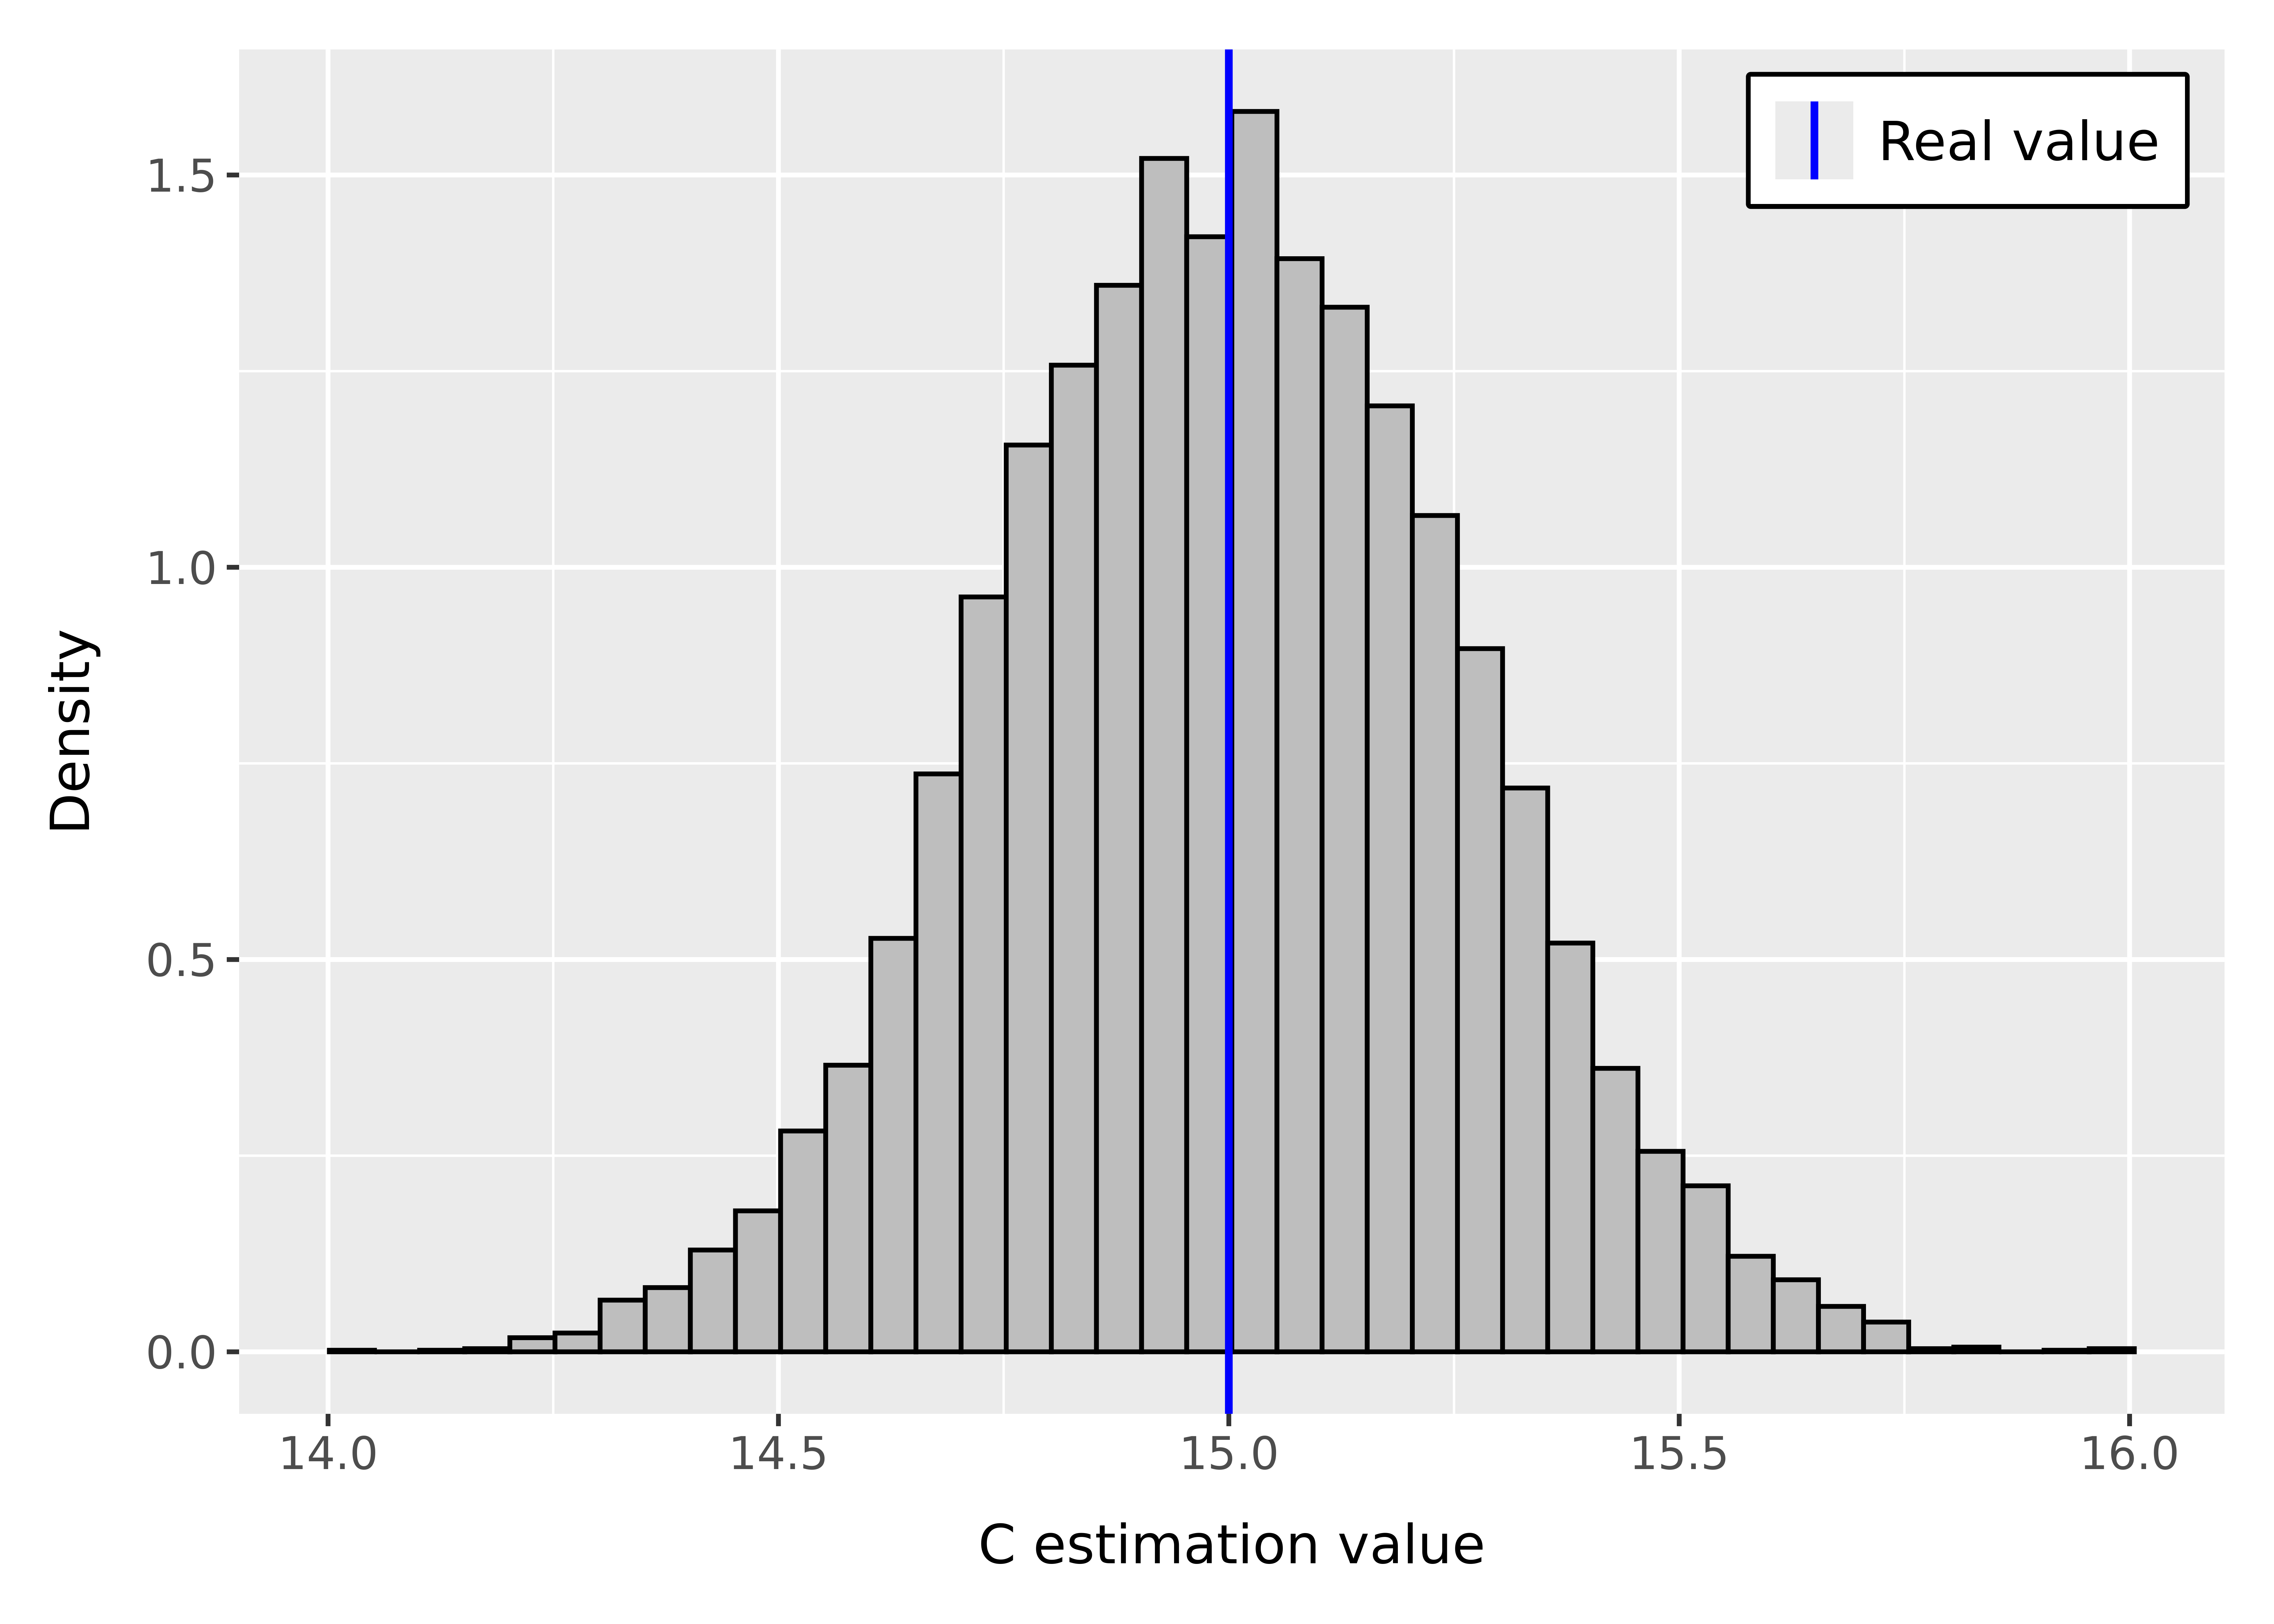
\includegraphics[width=1\linewidth]{Images/TRUE ERROR: NLS regression, n = 120.png}} б) Вибірка $n=120$
    \end{minipage}
    \hfill
    \begin{minipage}[H]{0.32\linewidth}
        \center{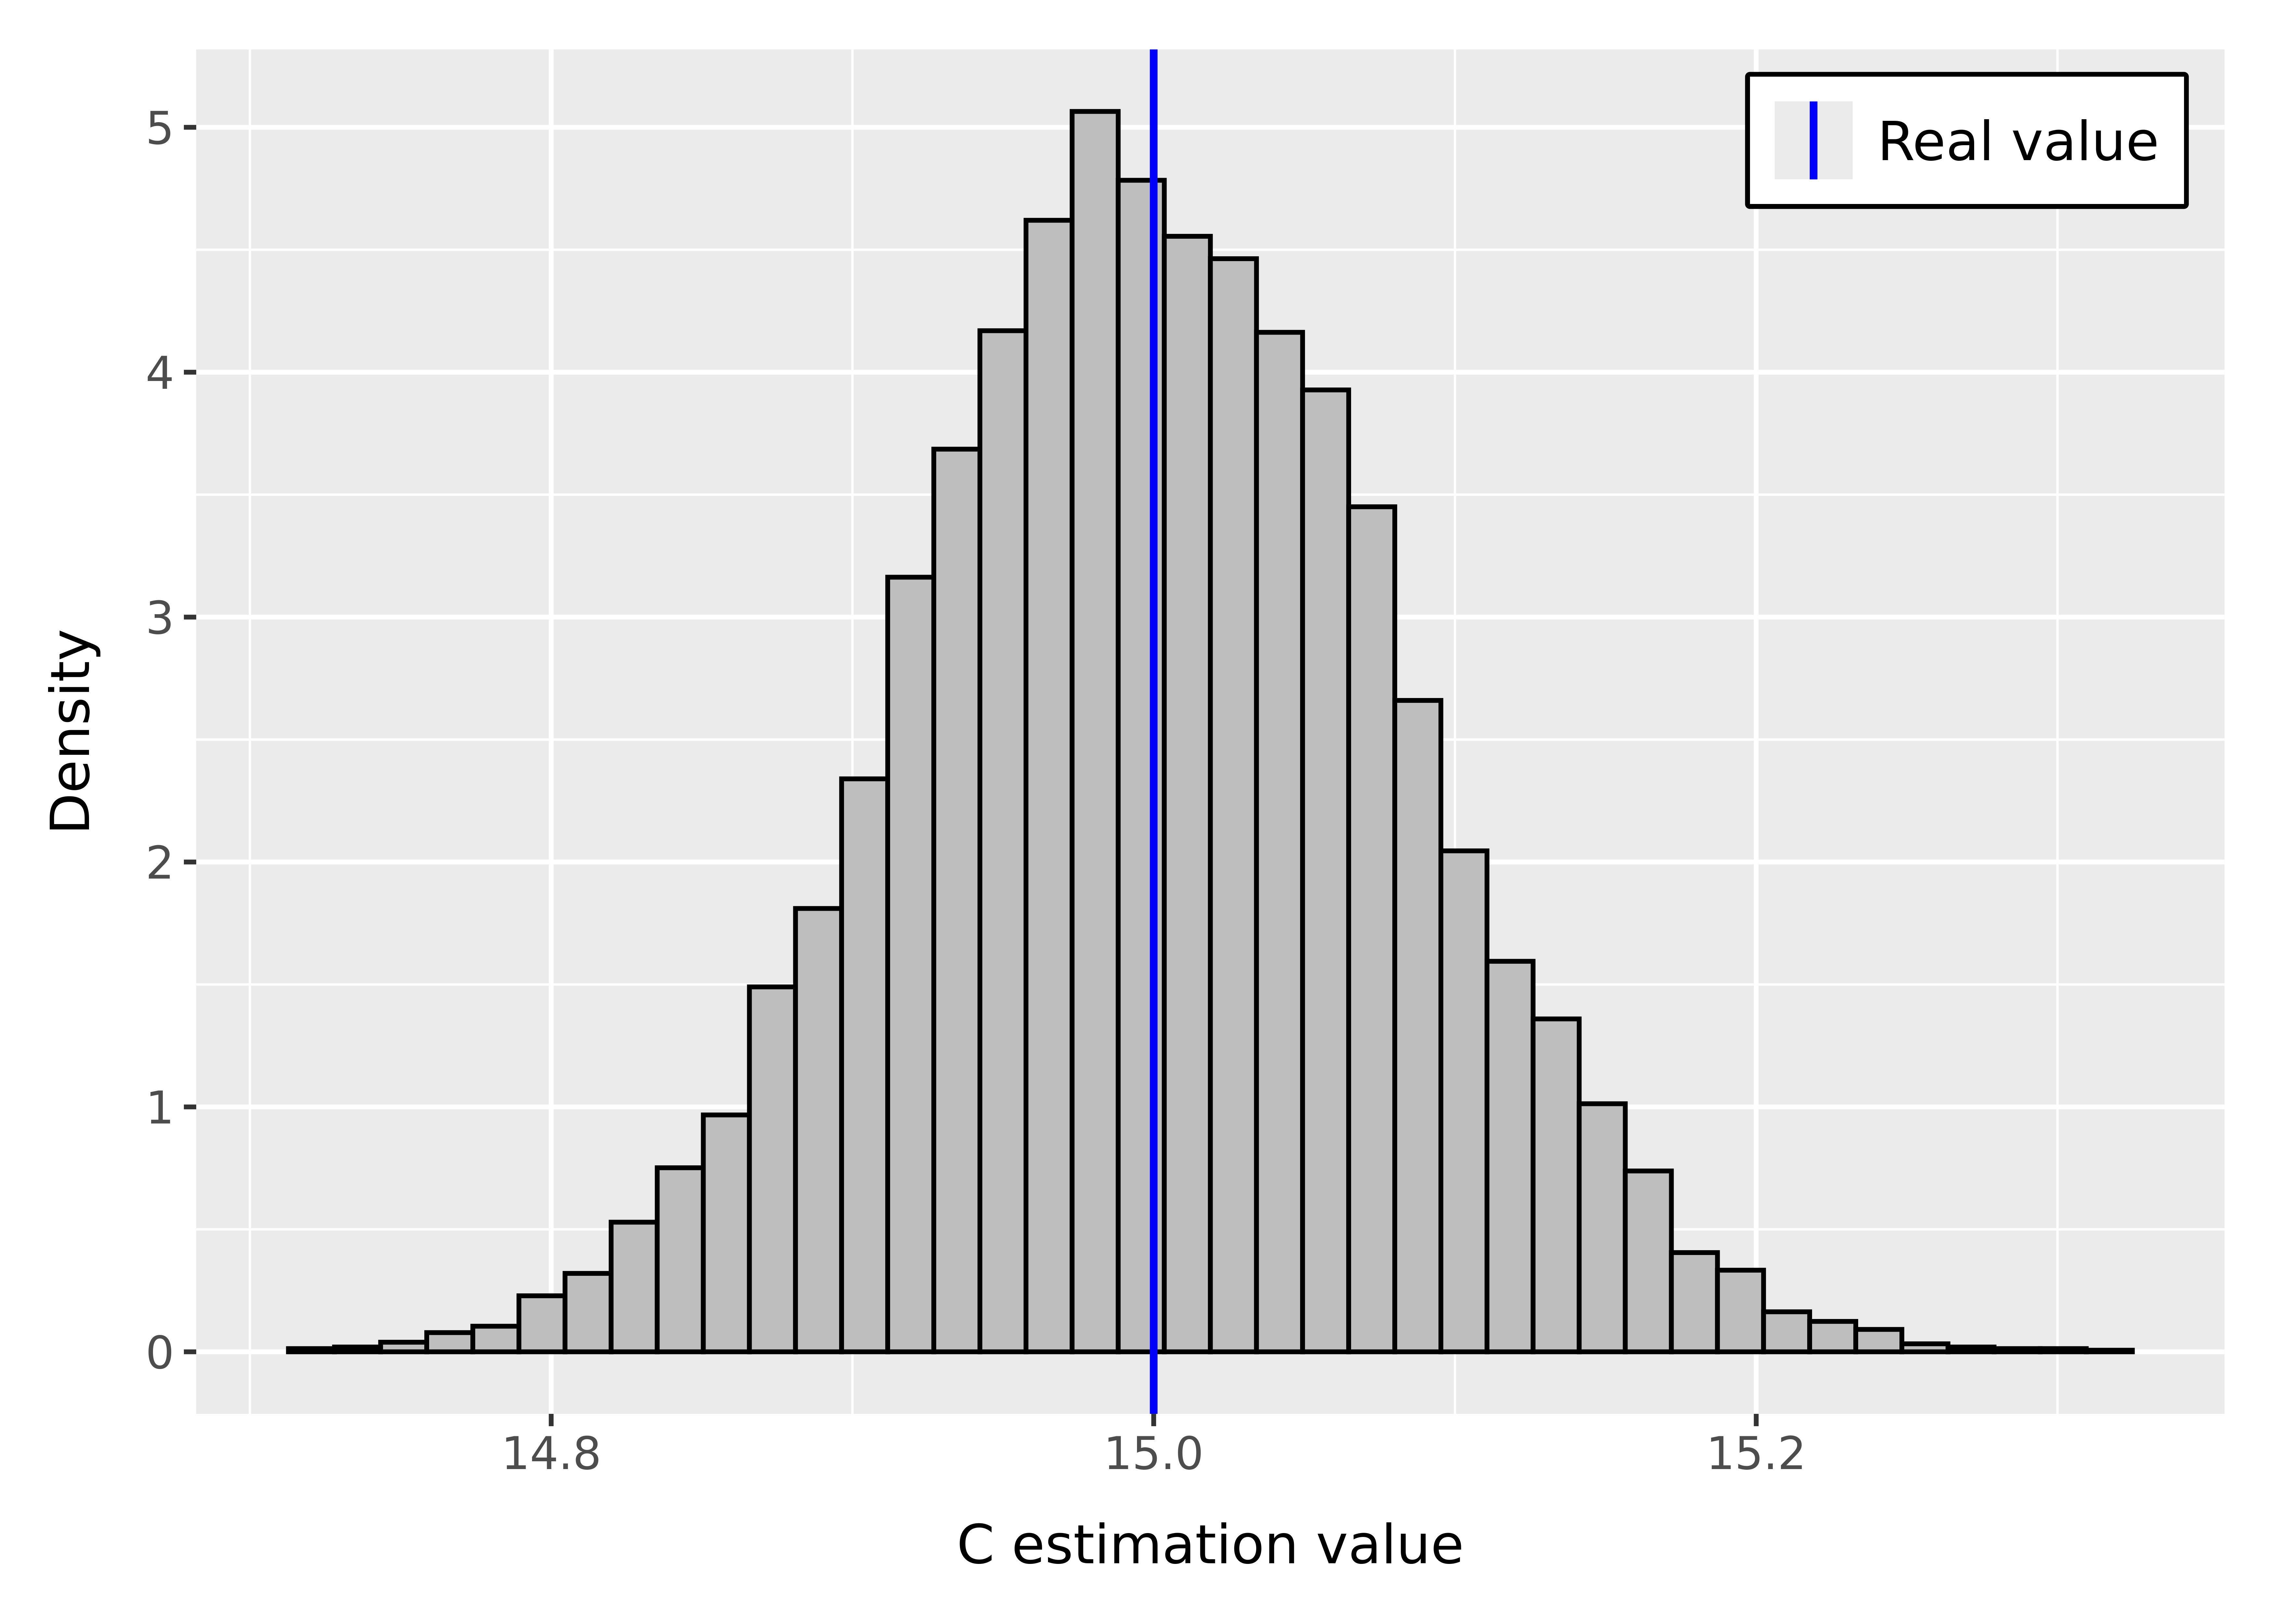
\includegraphics[width=1\linewidth]{Images/TRUE ERROR: NLS regression, n = 1200.png}} в) Вибірка $n=1200$
    \end{minipage}
    \caption{Результати серії з $N=10\,000$ повторних запусків МНК (глобальна адитивна помилки)}
    \label{pic: NLS true error results}
\end{figure}

\vspace{0.4cm}
\begin{table}[H]\centering
    \begin{tblr}{
            hlines={1pt,solid}, 
            vlines={1pt,solid},
            % hline{4-6}={1-5}{0pt},
            colspec={Q[3cm,c]Q[3cm,c]Q[3cm,c]Q[3cm,c]},
            cell{2}{2}={r=3,c=1}{c},
            % cell{1}{2}={r=1,c=2}{c},
            % cell{1}{4}={r=1,c=2}{c},
            row{2-4}={mode=math},
        }

        Розмір вибірки & Істинне значення & Вибіркове середнє & Стандартне відхилення \\
        n = 12         & 15               & 15.0097           & 0.8150                \\
        n = 120        & 15               & 15.0002           & 0.2572                \\
        n = 1200       & 15               & 15.0006           & 0.0814                \\

    \end{tblr}
    \caption{Статистичні характеристики серії з $N=10\,000$ повторних запусків МНК (глобальна адитивна помилка)}
    \label{table: NLS true error results}
\end{table}

Імплементація МНК засобами мови \texttt{R} за допомогою бібліотеки~\texttt{gslnls} наведена у Лістингу~\ref{code: NLS}.

\vspace{0.4cm}
\begin{lstlisting}[
    style           = myR,
    % backgroundcolor = {},
    caption         = {Запуск МНК для нелінійної регресіїної моделі~\eqref{eq: NLS true error energy intro}},
    label           = {code: NLS},
]
energy_dependency <- function(T, T0, A, B, C) {
    return(A + B * tanh((T - T0) / C))
}

data <- data.frame(
    T = as.vector(x_generated_points),
    y = as.vector(y_generated_points)
)

# Run nonlinear least-squares model
model_gslnls <- gsl_nls(
    fn = y ~ energy_dependency(
        T,
        T0 = input_parameters$T0,
        A = input_parameters$A,
        B = input_parameters$B,
        C
    ),
    data = data,
    algorithm = "lmaccel",
    start = c(C = 1)
)
\end{lstlisting}

\subsection*{Модель з локальною адитивною похибкою}
\addcontentsline{toc}{subsection}{Модель з локальною адитивною похибкою}

Нехай тепер задана ось така модель:
\begin{equation}\label{eq: NLS false error energy intro}
    E_i = A + B\tanh{\left( \frac{T_i-T_0}{C + \varepsilon_i} \right)},\ i=\overline{1,n},
\end{equation}
де значення~$A$, $B$ та $T_0$ є фіксованими (Табл.~\ref{table: NLS parameters}), величина~$C$ є невідомим параметром моделі, а випадкова похибка~$\varepsilon_i$ має нормальний розподіл:
\begin{equation}
    \varepsilon_i \sim \mathrm{N}(0,\sigma_c^2),\ i=\overline{1,n}
\end{equation}

Організація генерування даних у контексті моделі~\eqref{eq: NLS false error energy intro} аналогічна попередньому прикладу з глобальною адитивною похибкою. Однак, отримані результати свідчать про неспроможність МНК (Рис.~\ref{pic: NLS false error results}).

\begin{figure}[H]
    \begin{minipage}[H]{0.32\linewidth}
        \center{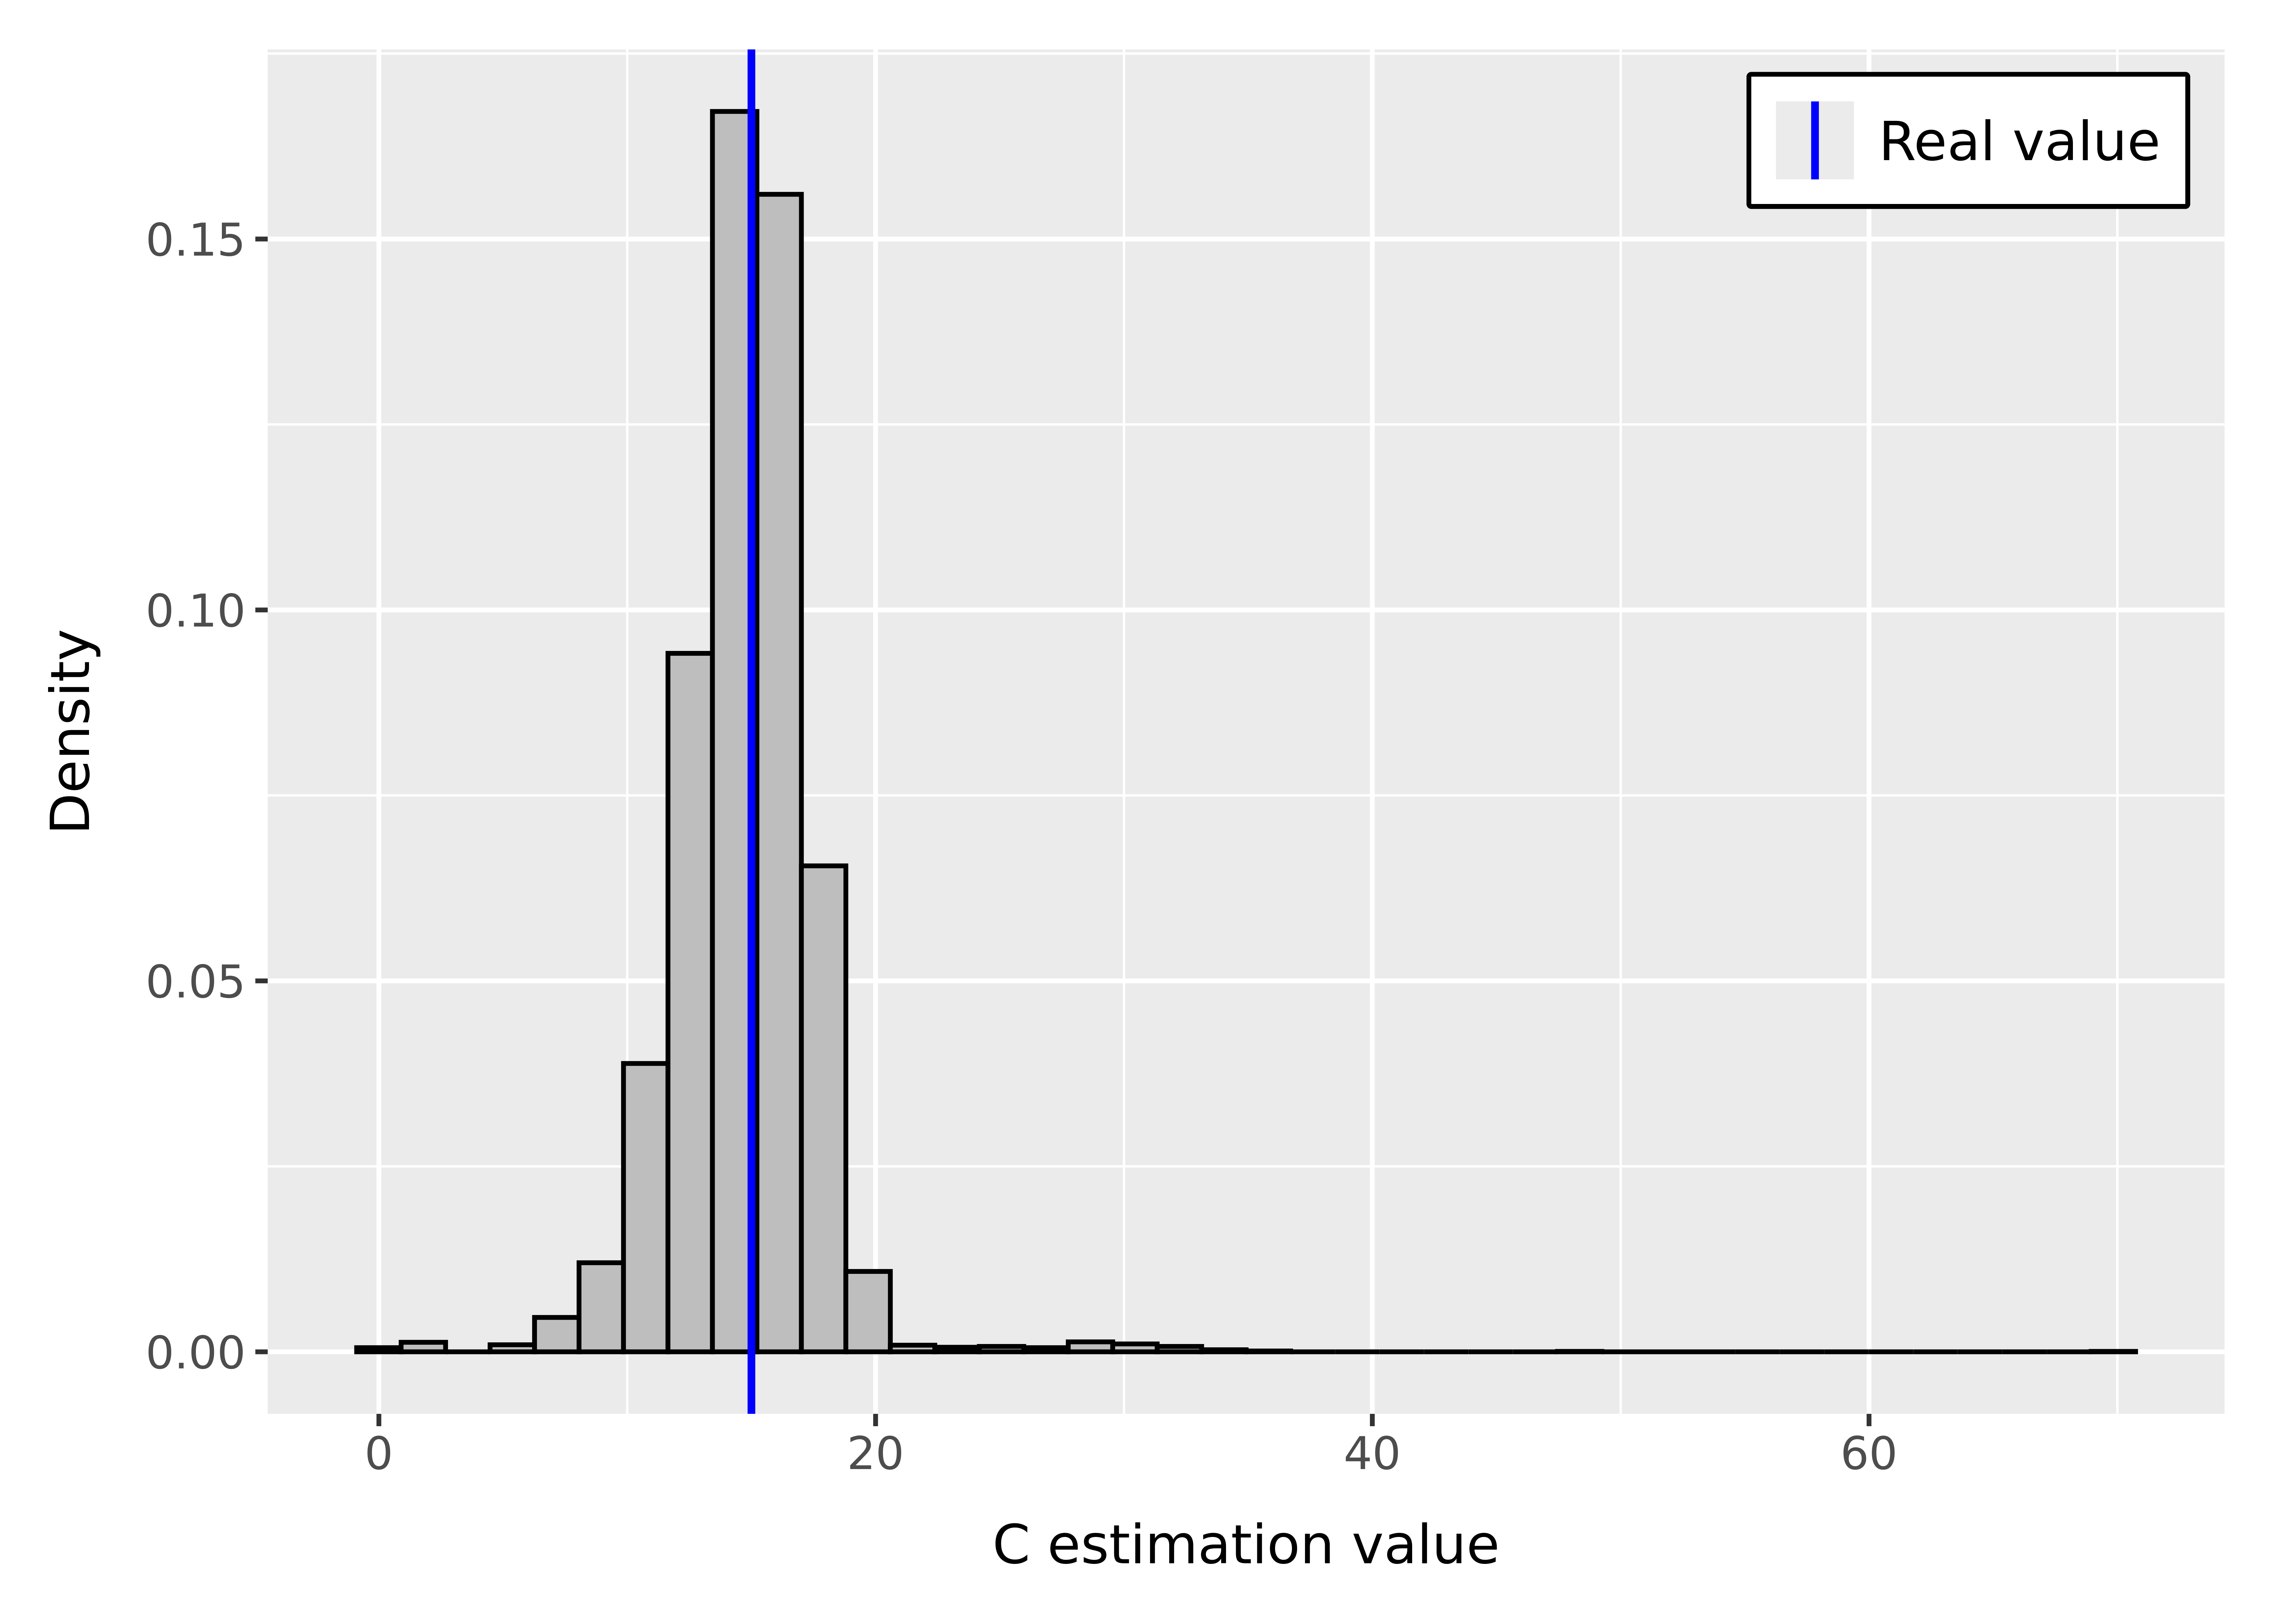
\includegraphics[width=1\linewidth]{Images/FALSE ERROR: NLS regression, n = 12.png}} а) Вибірка $n=12$
    \end{minipage}
    \hfill
    \begin{minipage}[H]{0.32\linewidth}
        \center{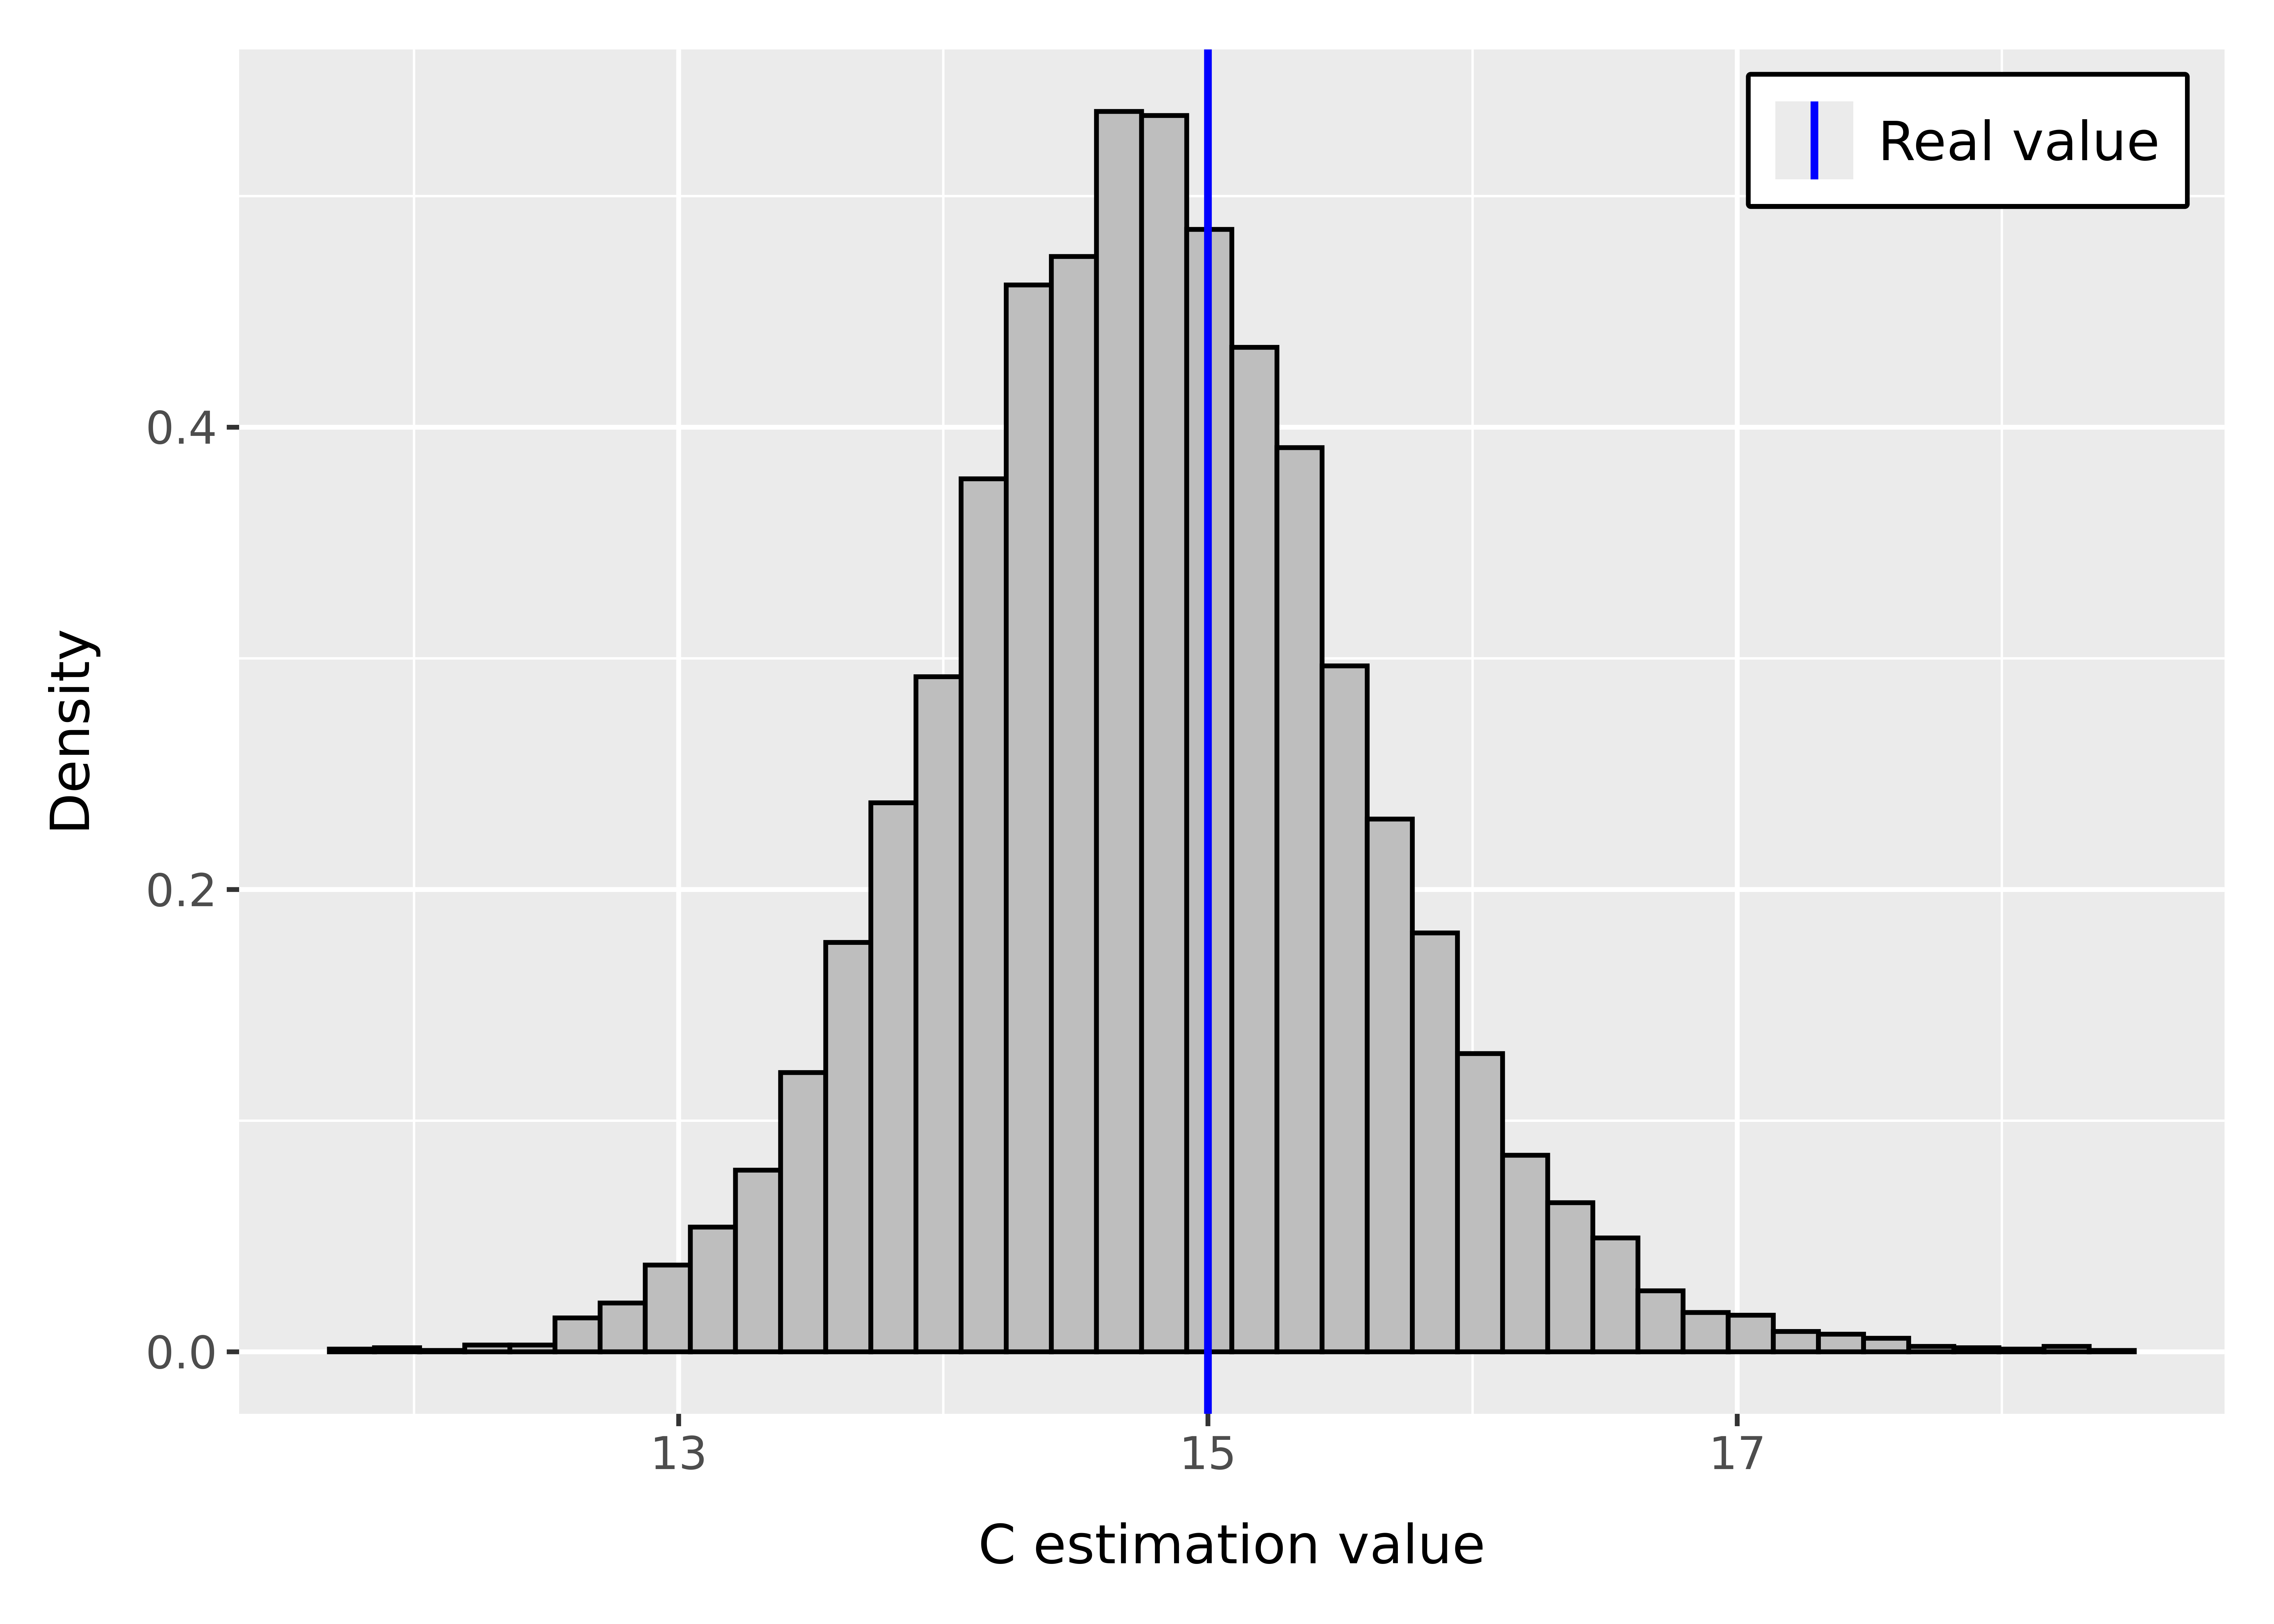
\includegraphics[width=1\linewidth]{Images/FALSE ERROR: NLS regression, n = 120.png}} б) Вибірка $n=120$
    \end{minipage}
    \hfill
    \begin{minipage}[H]{0.32\linewidth}
        \center{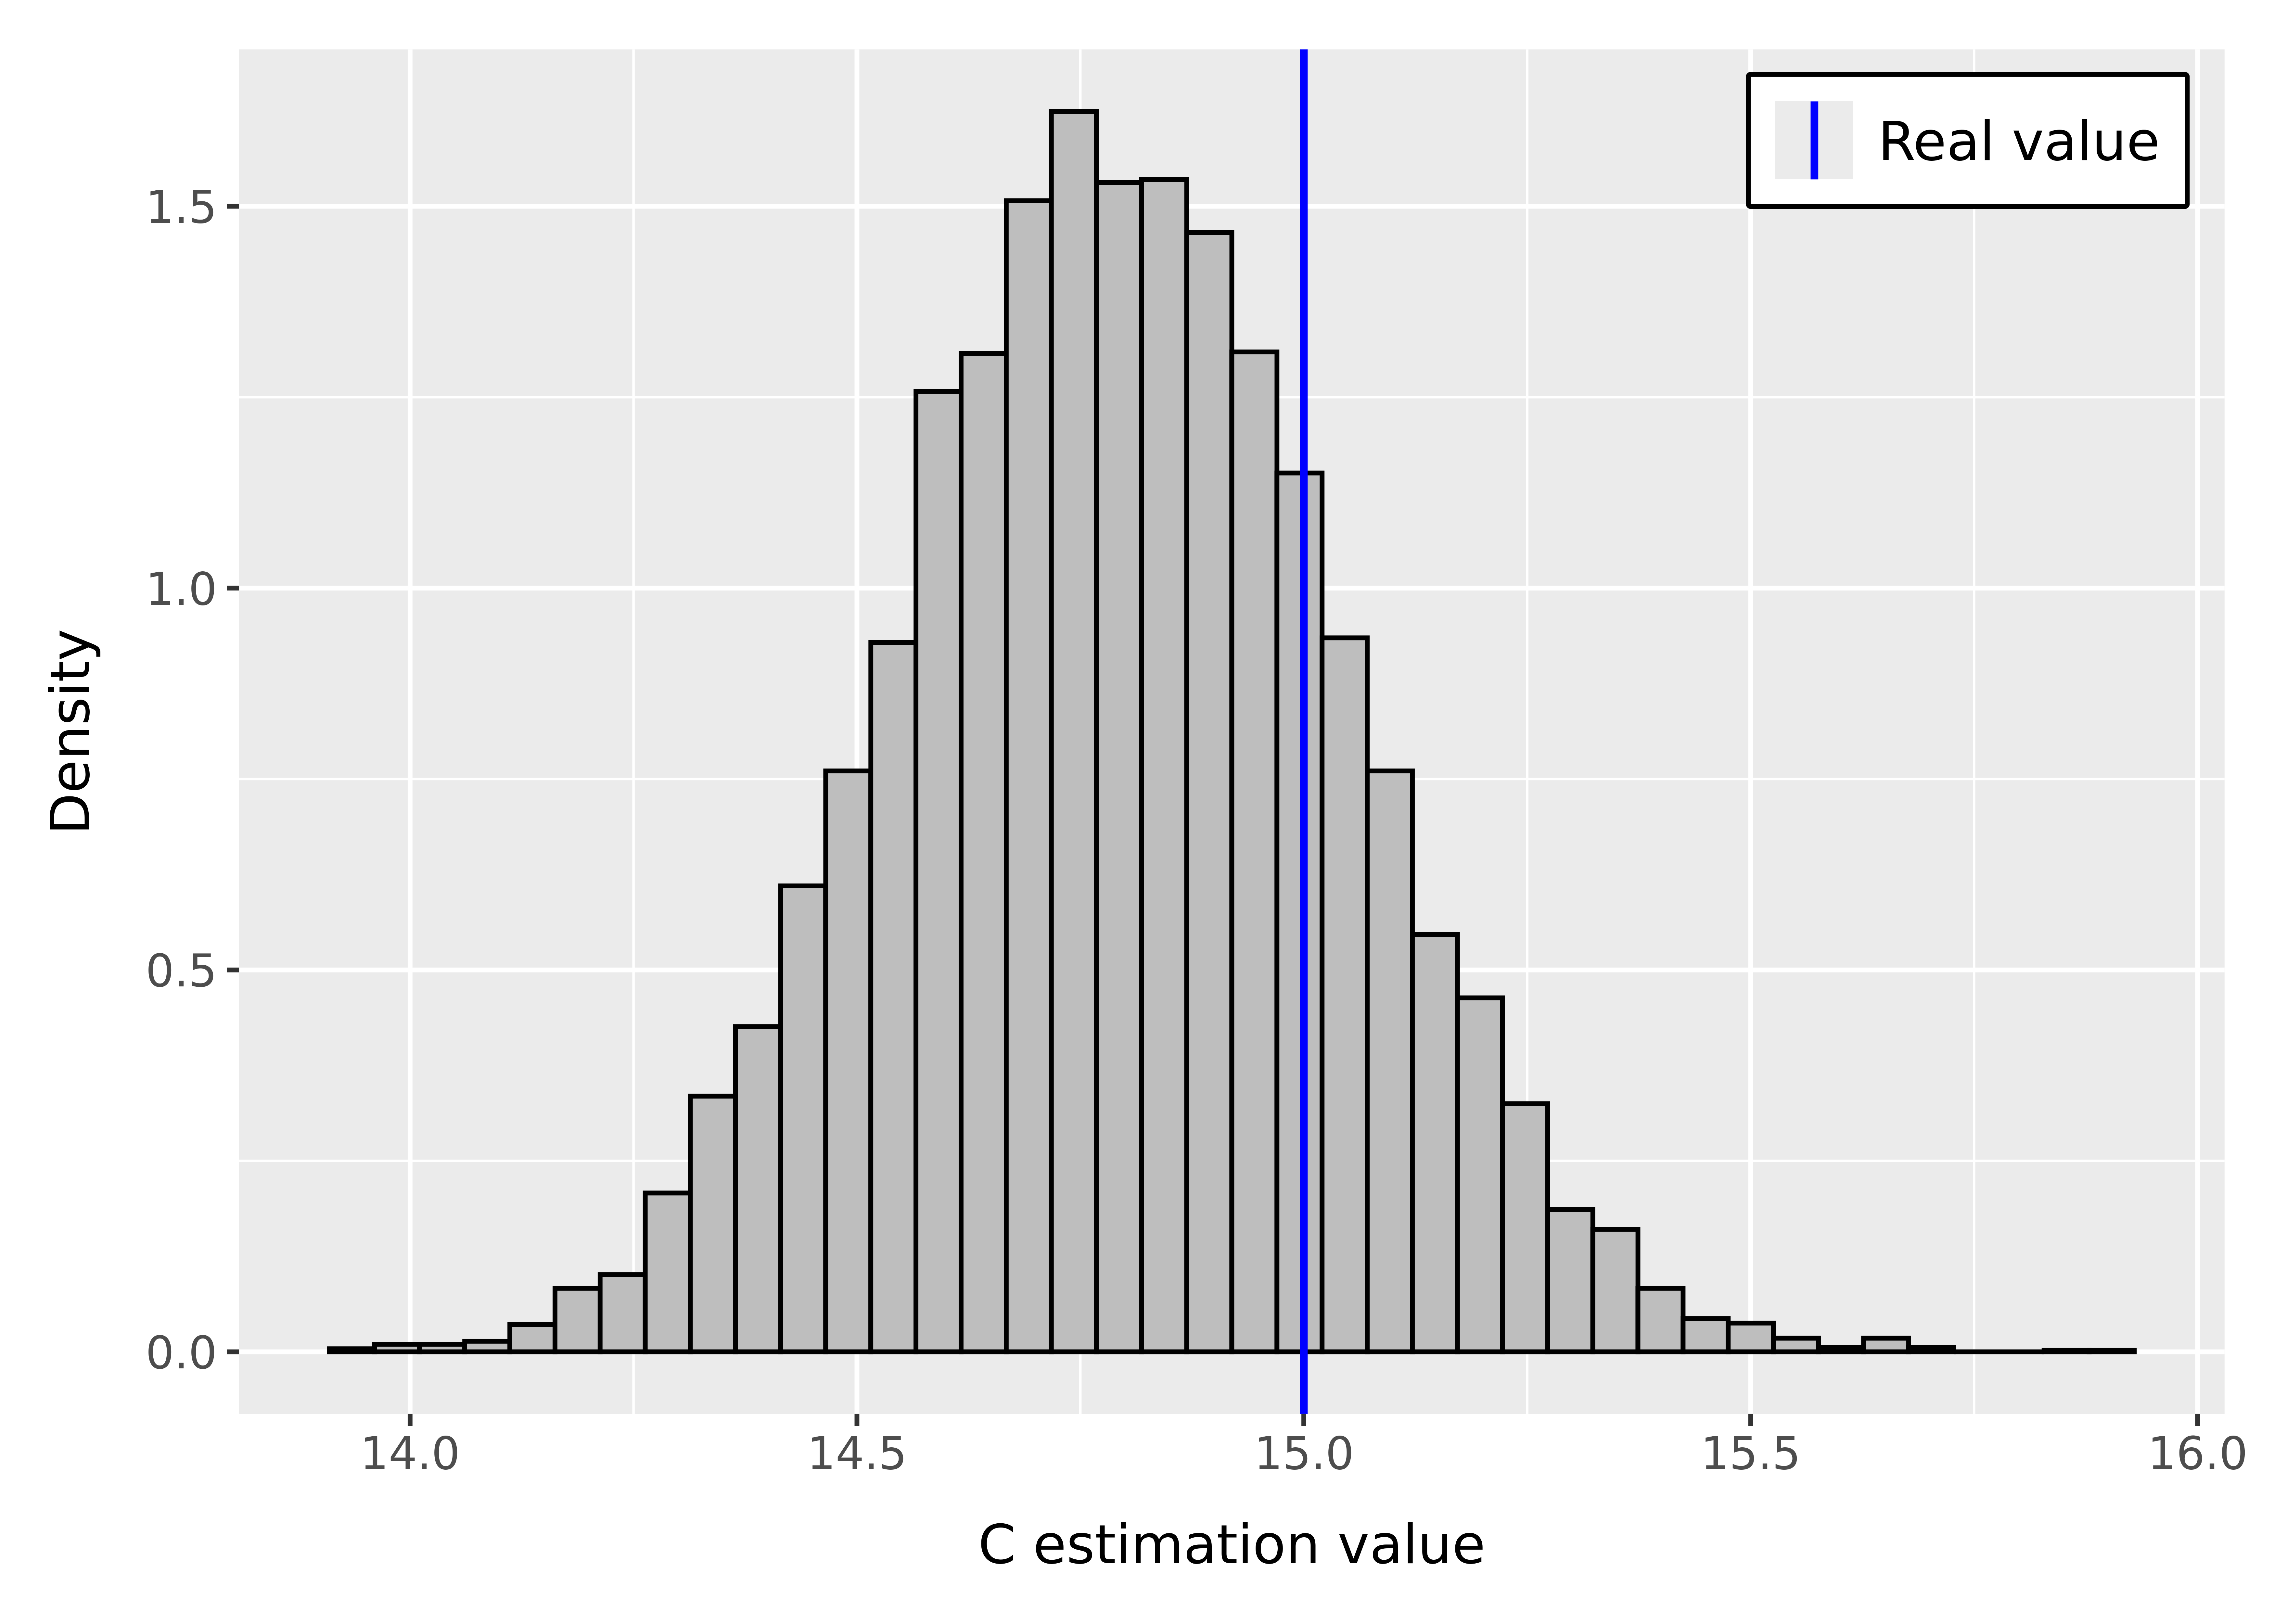
\includegraphics[width=1\linewidth]{Images/FALSE ERROR: NLS regression, n = 1200.png}} в) Вибірка $n=1200$
    \end{minipage}
    \caption{Результати серії з $N=10\,000$ повторних запусків МНК (локальна адитивна помилка)}
    \label{pic: NLS false error results}
\end{figure}

\vspace{0.4cm}
\begin{table}[H]\centering
    \begin{tblr}{
            hlines={1pt,solid}, 
            vlines={1pt,solid},
            % hline{4-6}={1-5}{0pt},
            colspec={Q[3cm,c]Q[3cm,c]Q[3cm,c]Q[3cm,c]},
            cell{2}{2}={r=3,c=1}{c},
            % cell{1}{2}={r=1,c=2}{c},
            % cell{1}{4}={r=1,c=2}{c},
            row{2-4}={mode=math},
        }

        Розмір вибірки & Істинне значення & Вибіркове середнє & Стандартне відхилення \\
        n = 12         & 15               & 14.7290           & 2.8841                \\
        n = 120        & 15               & 14.7791           & 0.7993                \\
        n = 1200       & 15               & 14.7945           & 0.2491                \\

    \end{tblr}
    \caption{Статистичні характеристики серії з $N=10\,000$ повторних запусків МНК (локальна адитивна помилка)}
    \label{table: NLS false error results}
\end{table}

\newpage
\printbibliography[title={Перелік посилань}] % \nocite{*}
\addcontentsline{toc}{section}{Перелік посилань}

\end{document}